%!TEX root = paper.tex
%%%%%%%%%%%%%%%%%%%%%%%%%%%%%%%%%%%%%%%%%%%%%%%%%%%%%%%%%%%%%%%%%%%%%%%%%%%%%%%%
\section{Characterising Platforms and Games}
\label{sec:background}

This section covers the basic characteristics of different gaming platforms, including digital storefronts that sell copies of games for local use, and Cloud gaming approaches where the game is executed and rendered ``in the cloud'' (i.e. in remote datacenters), and an audio/video stream is sent back to the player. We also present observations about the properties of the games offered.
Section~\ref{sec:engagement} will then use these characteristics to reason about player engagement and budget considerations.

%%%%%%%%%%%%%%%%%%%%%%%%%%%%%%%%%%%%%%%%%%%%%%%%%%%%%%%%%%%%%%%%%%%%%%%%%%%%%%%%
\subsection{Platform Characteristics}

Below we examine currently active (cloud and other) gaming platforms with regards to pricing models, and hardware requirements and costs. The information presented was collected between July 2015 and February 2016. All costs are from an European, specifically German, perspective. If a product is not available in this region, the prices are converted using the most recent currency exchange rates.


\subsubsection{Video Game Consoles}

A classical approach to video gaming is using dedicated consoles with physical copies of game media (e.g., a data DVD) bought at a retailer. The price for (non-portable) consoles varies but usually lies between \SI{300}[\EUR] and \SI{400}[\EUR] for the latest console generation, i.e., \textit{Wii U}, \textit{PlayStation 4}, and \textit{Xbox One}. New, major game releases are mostly priced at either \SI{60}[\EUR] or \SI{70}[\EUR]. Once on the market, the game prices decrease rather slowly. In recent years, retail stores have been complemented with console-specific, proprietary digital distribution services that also offer the latest game at the full price. These official stores are usually exclusive vendors for digital game codes where competitors are excluded.

%, meaning that there will be no competition that quickly reduces prices.

Subscriptions fees often apply for the multiplayer mode of games, e.g., \textit{PlayStation Plus} or \textit{Xbox Live Gold} with annual prices of \SI{50}[\EUR] and \SI{60}[\EUR], respectively. These services also include a small, monthly changing palette of older game titles.

% generally offer a monthly rotating palette of (older or smaller) game titles included in the subscription.

% \paragraph{Historical Example: OnLive}


\subsubsection{The PC Gaming Ecosystem}
\label{sec:pcgaming}

The rise of easy-to-use digital distribution platforms and the independent (``indie'') game scene reinvigorated PC gaming just a few years ago. Today, PC gaming is dominated by large digital marketplaces, and the \steam platform in particular. The platform has about $10$ million concurrent users at every time of day. It periodically offers large, often seasonal, sales of recent games at greatly reduced prices (rebates of 75\% for a year-old game are not uncommon). In addition, many resellers offer digital codes for other platforms, often at much lower prices. Alternative storefronts, entirely independent from \steam, also exist, such as \textit{GOG}\footnote{\url{https://www.gog.com/}}.%, and enrich the competition even more.

The official prices for new major releases on PC are comparable to those of console titles. However, due to the competition between marketplaces, the street prices are significantly lower even at launch, and also drop more quickly. Another recent trend are bundles of games, especially prevalent in the indie games scene, which are offered for either a low price or, more commonly, with a pay-what-you-want model with parts of the money going to charities. \textit{Humble Bundle}\footnote{\url{https://www.humblebundle.com/}} is a prominent example. % Number of games >>> what consoles have

Hardware viable for PC gaming starts at about \SI{500}[\EUR] but has practically no upper limit for enthusiasts (especially the \gls{GPU} is a cost driver, but essential for modern  PC gaming). Thus, the barrier for customers to start PC gaming is higher than for consoles, which is, however, compensated by an increased flexibility and longevity of hardware.

%albeit with increased flexibility and longevity. Hardware viable for PC gaming starts at about \SI{500}[\EUR] but has practically no upper limit for enthusiasts. The main spender will usually be the \gls{GPU}, often surpassing the \acrshort{CPU} in its performance impact in today's games by far.

%recurring bundles/subscriptions (humble monthly)
%	console/netflix similarities

% Steam Sales:
% Large seasonal sales (christmas, summer, lunar new year, halloween, fall, spring, ...) of many/most games on the platform usually rebates of 50\% and up.
% Weekly sales
% Daily sales
% Weekend sales
% Free weekends


\subsubsection{Geforce NOW}

\textit{Geforce NOW}\footnote{\url{http://shield.nvidia.com/game-streaming-with-geforce-now}} This Cloud Gaming service is available in North America and selected European countries. In Germany the service currently offers $68$ PC titles for a monthly subscription fee of \SI{10}[\EUR]. An additional per-game one-time fee between \SI{13}[\EUR] and \SI{60}[\EUR] is charged for the access to the $19$ most prominent and recent games. The service is delivered from six specialized data center locations (Dublin and Frankfurt in Europe).

The requirements to use this service are rather steep, demanding \SI{50}{\mega\bit\per\second} for a full 1080p60\footnote{\label{foot:rate}Please note: This frame rate of \SI{60}{\hertz} represents the rate of the video encoder and not the game's actual frame rate, which might be considerably lower depending on the complexity of the game.} stream (\SI{10}{\mega\bit\per\second} in order to use the service at all) and a maximum \acrshort{RTT} of \SI{60}{\milli\second} to one of the data centers. In addition, streaming is exclusive to NVIDIA's \textit{SHIELD} devices which start at \SI{200}[\EUR].

% Started in parts of Europe in Q4/2015


\subsubsection{Playstation Now}

Sony's Cloud gaming service offers to stream titles from previous PlayStation generations, as the latest console generation lacks backwards compatibility. It is currently available in North America and the UK, with a closed beta running in  other European countries and Japan.

The offered titles and exact pricing vary from country to country. For the UK, about $190$ titles are available, and most titles are covered by the monthly subscription fee of about \SI{17}[\EUR]. All titles are also available through a separate rental service, costing about \SI{4}[\EUR] for \SI{48}{\hour} and \SI{10}[\EUR] for one month of access. This is in addition for the device cost, as the service is only available on  PlayStation 4 and 3 consoles as well as some select Sony TVs and other devices with extra game controller.

%(which would however necessitate the purchase of a game controller).

The streaming itself is performed at a resolution of 720p60\cref{foot:rate} requiring a \SI{5}{\mega\bit\per\second} connection. Reports on the video quality have been rather mixed.\footnote{\url{http://www.eurogamer.net/articles/digitalfoundry-2015-hands-on-with-playstation-now}} % Sony is also reportedly using specialized server hardware, adapted from regular PlayStation 3s, effectively eliminating any chance for multi-purpose uses of these devices. This could lower scalability gains.

% cost and some more infos:
% http://www.pocket-lint.com/news/126394-playstation-now-subscription-service-comes-to-the-uk-what-is-it-and-how-can-you-get-it

% (US/UK only?) Deuschlandbeta seit ~Q4/2015



%%%%%%%%%%%%%%%%%%%%%%%%%%%%%%%%%%%%%%%%%%%%%%%%%%%%%%%%%%%%%%%%%%%%%%%%%%%%%%%%
\subsection{Characteristics of Games}

Following the discussion of gaming platform characteristics, we now turn our attention to the properties of the games offered on the various platforms: number of games, prices, ages, play lengths, and review scores. Table~\ref{tab:game-stats} provides an overview of the data.

%of the cost-benefit analysis is
%\todo[inline]{PZ: Naive but not untrue. What is engagement in this context? Is engagement the value metric?}
%The leading question for investigating the customer side is ``How can we properly estimate the (perceived) value of a service for the customer?'' where the perceived value deserves a definition and specific attention. This is targeted by the means of assessing the user engagement. Simply counting the number of games available for a specific service or for a specific amount of money may be the easiest value metric but may also fall short, as the enjoyment of a specific game can be very subjective. However, with the help of further metrics  a more objective impression of the popularity and the value of individual titles can be formed. 
In order to investigate these characteristics, data was collected from multiple sources and merged into a consistent data base. In the interest of repeatability and reproducibility, all of the data reported on in this work, and all of the code used to collect and process it, can be found in public repositories\footnote{The main repository can be found at \url{https://github.com/mas-ude/cost-of-cloud-gaming}}. Please note that due to space constraints and the multidimensional nature of the dataset, we can only present a limited number of findings in this paper.

%Both these attributes usually play a role in one's decision to play a certain game. 

%with an additional question of ``What is the definition of value in this context?''. To answer these some means to meter user engagement is required, as this represents the core of those questions. Simply counting the number of games available for a specific service or for a specific amount of money may be the easiest value metric but may also fall short, as the enjoyment of a specific game can be very subjective.

% %!TEX root = paper.tex

\begin{table}
\caption{Metadata for the \steam, \metacritic, \hltb, \psnow, and \gfnow datasets. Records with a * note include games from other platforms than PC, PlayStation, and GeForce Shield.}
\label{tab:dataset-metadata}
\centering
\begin{tabu}{X[1.5]|X[r]|X[0.7,r]|X}
\toprule
Product & Date generated & \# of records & Method of generation\\
\midrule
\steam & 2015-07-14 & \num{5996} & Steam \& SteamSpy\\
\steam & 2015-10-30 & \num{6769} & Steam \& SteamSpy\\
\steam & 2016-02-06 & \num{7749} & Steam \& SteamSpy\\
\psnow & 2016-02-09 & \num{190} & Official list\\
\gfnow & 2016-02-12 & \num{69} & Manual screen scraping\\
\metacritic & 2016-03-02 & * \num{46197} & Web scraping\\
\hltb & 2016-03-01 & * \num{18433} & Web scraping\\
\bottomrule
\end{tabu}
\end{table}

% %!TEX root = paper.tex

\begin{table*}
\centering
\caption{Overview of datasets. Values with * are 99th percentiles chosen due to unrealistically large outliers.}
\label{tab:dataset-stats}
\begin{tabular}{c|c|r|r|r|r|r|r}
Dataset & Metric & Mean & Min & 1Q & Median & 3Q & Max\\
\hline
\hline
\steam & Number of records & \num{7749} & -- & -- & -- & -- & -- \\
\steam & Owners & \num{218112} & \num{0} & \num{4831} & \num{21740} & \num{107299} & \num{58666968} \\
\steam & players 2weeks & \num{9064} & \num{0} & \num{0} & \num{509} & \num{1526} & \num{7860554} \\
\steam & players forever & \num{138322} & \num{0} & \num{1780} & \num{9408} & \num{51997} & \num{58666968} \\
\steam & Average playtime (forever) & \num{507} & \num{0} & \num{93} & \num{200} & \num{429} & \num{45540} \\
\steam & Median playtime (forever) & \num{246} & \num{0} & \num{36} & \num{101} & \num{216} & \num{67538} \\
\steam & average 2weeks & \num{144} & \num{0} & \num{0} & \num{48} & \num{173} & \num{11387} \\
\steam & median 2weeks & \num{126} & \num{0} & \num{0} & \num{35} & \num{128} & \num{11387} \\
\steam & Price & \num{564} & \num{-1.26} & \num{0.99} & \num{3.39} & \num{7.49} & \num{119.00} \\
\hline
\psnow & Number of records & \num{252} & -- & -- & -- & -- & -- \\
\psnow & Rental fee for 4 hours & \num{3.02} & \num{1.99} & \num{1.99} & \num{2.99} & \num{2.99} & \num{22.99} \\
\psnow & Rental fee for 7 days & \num{5.48} & \num{1.99} & \num{3.99} & \num{4.99} & \num{5.99} & \num{14.99} \\
\psnow & Rental fee for 30 days & \num{8.40} & \num{3.99} & \num{5.99} & \num{6.99} & \num{7.99} & \num{22.99} \\
\psnow & Rental fee for 90 days & \num{12.57} & \num{3.99} & \num{7.99} & \num{8.99} & \num{14.99} & \num{49.99} \\
\hline
\gfnow & Number of records & \num{68} & -- & -- & -- & -- & -- \\
\gfnow & Price & \num{6.98} & \num{0} & \num{0} & \num{0} & \num{13.99} & \num{59.99} \\
\hline
\metacritic & Number of records & \num{45803} & -- & -- & -- & -- & -- \\
\metacritic & User score & \num{6.9} & \num{0} & \num{6.2} & \num{7.3} & \num{8.1} & \num{9.3} \\
\metacritic & Score & \num{69} & \num{8} & \num{62} & \num{72} & \num{79} & \num{96} \\
\hline
\hltb & Number of records & \num{18129} & -- & -- & -- & -- & -- \\
\hltb & Main story length & \num{26} & \num{0.02} & \num{2.5} & \num{6} & \num{12} & * \num{94} \\
\hltb & Main extra length & \num{21} & \num{0.08} & \num{5} & \num{10} & \num{20} & * \num{126} \\
\hltb & Completionist length & \num{28} & \num{0.03} & \num{5} & \num{13} & \num{29} & * \num{250} \\
\hltb & Combined length & \num{13} & \num{0.02} & \num{3} & \num{8} & \num{15} & \num{420} \\
\end{tabular}
\end{table*}

\todo[inline]{PZ: Viele daten, aber welche plattform ist die beste?}


%%%%%%%%%%%%

\begin{table*}
\centering
\caption{Game characteristics on the investigated platforms. Title counts and price data from Web/API/screen scraping, lengths from \hltb, ages and review scores from \metacritic. (\psnow prices are time-rental based and thus omitted).}
\label{tab:game-stats}
	\begin{tabu}{X[2]|X[r]X[r]X[r]X[r]X[r]X[r]X[r]X[r]X[r]}
	\toprule
	Service & Titles & Age $\mu$ & Age $\sigma$ & Length $\mu$ & Length $\sigma$ & Score $\mu$ & Score $\sigma$ & Price $\mu$ & Price $\sigma$\\
	\midrule
	\gfnow & $68$ & \SI{2.87}{\year} & \SI{1.95}{\year} & \SI{14.65}{\hour} & \SI{14.44}{\hour} & $75.9$ & $9.44$ & $6.98$ & ---?---\\
	\psnow & $252$ & \SI{5.24}{\year} & \SI{2.55}{\year} & \SI{12.26}{\hour} & \SI{15.47}{\hour} & $76.72$ & $11.43$ & --- & ---\\
	\steam & $7749$ & \SI{3.36}{\year} & \SI{3.95}{\year} & \SI{13.02}{\hour} & \SI{20.49}{\hour} & $71$ & $12$ & $5.64$ & ---?---\\
	\bottomrule
	\end{tabu}
\end{table*}


%%%%%%%%%%%%
\subsubsection{Number of Games}

This basic metric quantifies the range of games on offer. The two Cloud platforms offer a very limited number of games when compared to the games available on \steam, which itself again only represents a subset of all games available either on the PC platform (\metacritic lists $16192$) or across all platforms ($45803$ listed on the site). Two possible, simple explanations for the low game count on the Cloud platforms come to mind: One is that they were launched relatively recently in comparison to \steam (2003). Two, the choice of games for a Cloud gaming platform is necessarily curated by the platform operator: The operator guarantees that all of the offered games do indeed can run on the Cloud's hardware, and are usable across the network at a satisfying level of quality. This burden shifts to the end user for digital storefronts like \steam, allowing these platforms to offer a larger variety of games, including ones that are very demanding on the hardware.


%%%%%%%%%%%%
\subsubsection{Game Ages}

The average age of games, as computable from their release dates, appears to be  relatively high for all of the investigated platforms, and particularly so for \psnow. However, the standard deviations ($\sigma$) indicate that these numbers should be interpreted carefully. First, \psnow might be considered a special case, as it is specifically advertised as a backwards compatibility for older, pre-PlayStation 4 games that do not run on the latest Sony platform any more. For \steam, we observe from the data that the distribution is significantly skewed towards recent titles (with the median below $15$ months), and sports a long tail that extends beyond $25$ years (due to re-releases of ``classic'' games on the platform).


%%%%%%%%%%%%
\subsubsection{Game Lengths}

Game publishers are usually not outspoken about the intended playthrough length of games (nor do all games necessarily end). However, players may self-report their experienced playthrough times on sites like \hltb\footnote{\url{http://howlongtobeat.com/}}, on whose data this analysis is based\footnote{\url{https://github.com/mas-ude/gamelengths-scraper}}. Reported times are separated into different play styles, e.g., ``main story'' for players that just finish the main objectives of a game, or ``completionist'' for those who explore the game to the fullest extent. Only an aggregate time over all reports per play style is shown for every game. (For our analysis, we average over all play styles for every game.) %It should however be stressed again, that this is a self-reporting site without strong validity checks, which has to be considered when contemplating the accuracy of the data.
Figure~\ref{fig:gamelengths-violin} shows the distribution of game lengths for the three platforms under investigation, and an ``overall'' distribution that includes further platforms and gaming systems. Among the three platforms, the mean and median reported game lengths (approximately $14$ hours) are largest for \gfnow. In contrast to the curated choice of games on the Cloud systems, \steam also offers shorter and longer games.


\begin{figure}[!t]
	\centering
	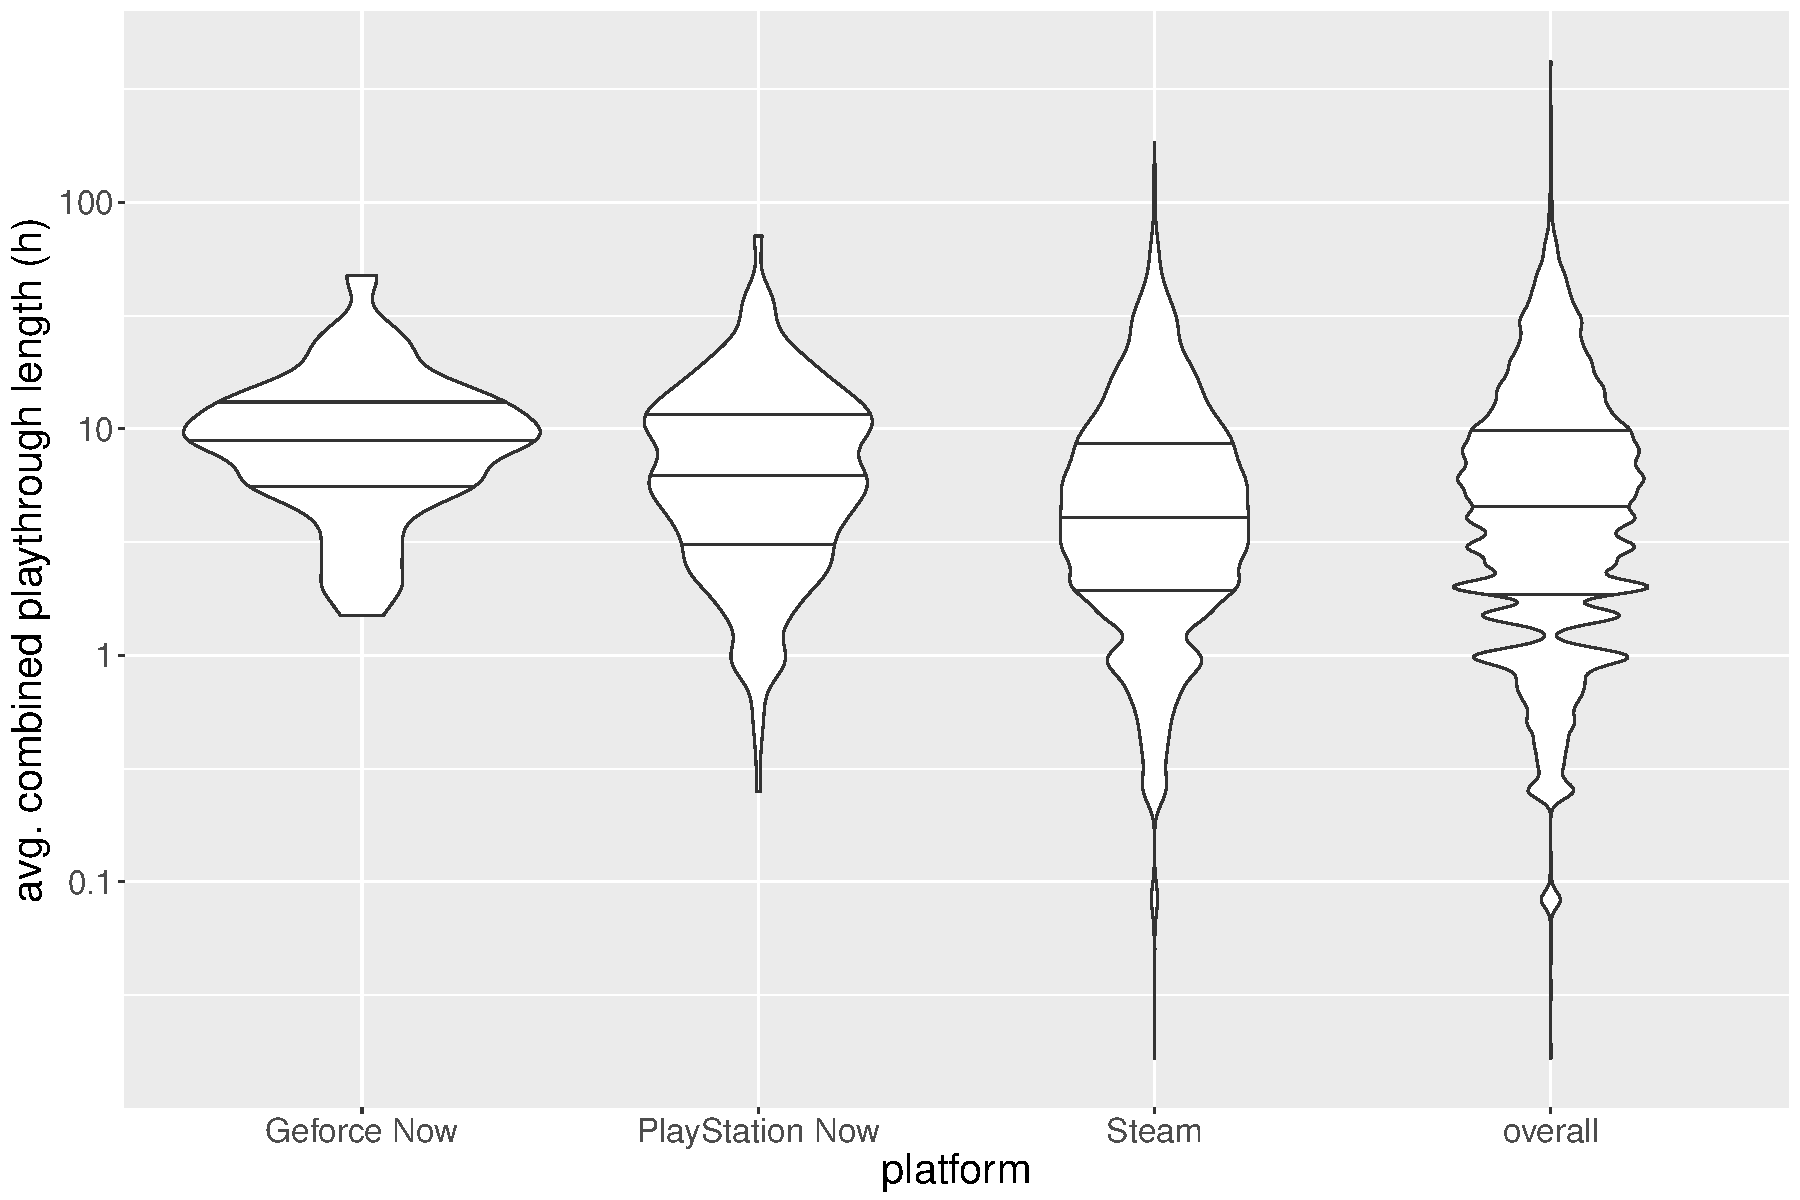
\includegraphics[width=1.0\columnwidth]{images/gamelengths-by-platform-violin.pdf}
	\caption{Violin plot of the per-platform average game lengths from \hltb, aggregated over all play styles. The number of games per bin are $68$, $209$, $7764$, and $18433$.}
%	aggregated over all play styles (raw data source: \hltb).}
\label{fig:gamelengths-violin}
\end{figure}



\todo[inline]{AR: Now with 100\% less ``ownership'' discussion!}
An initial grasp of the popularity of individual titles can often be derived from its price as well as the number of owners. Few platforms however publish sales numbers, though a few recurring studies on retail sales exist. For this work however, data from the \steam platform was used\footnote{\url{https://github.com/mas-ude/steam-data-stats}}. Using the official \acrshort{REST} \acrshort{API} the name and the current price of each game was fetched at three different points in time. While details on the pricing are later on discussed around Table~\ref{1tab:dataset-stats}, we can on a high level acknowledge the different prices obtained during sale and non-sale periods.
\todo[inline]{PZ: The reference to the far away table shows a structural issue, which might be fixed with the reorganisation suggested by AR.}

%where sale periods, e.g., the Lunar New Year Sale, yield substantially different prices.

% On a high-level, the sale periods shine out 

%The influence of sales periods can be easily observed in the \acrshort{CDF} of prices in Fig. \ref{fig:steam-prices}, where the data from February was collected during \steam's Lunar New Year Sale.

%\begin{figure}[!t]
%	\centering
%	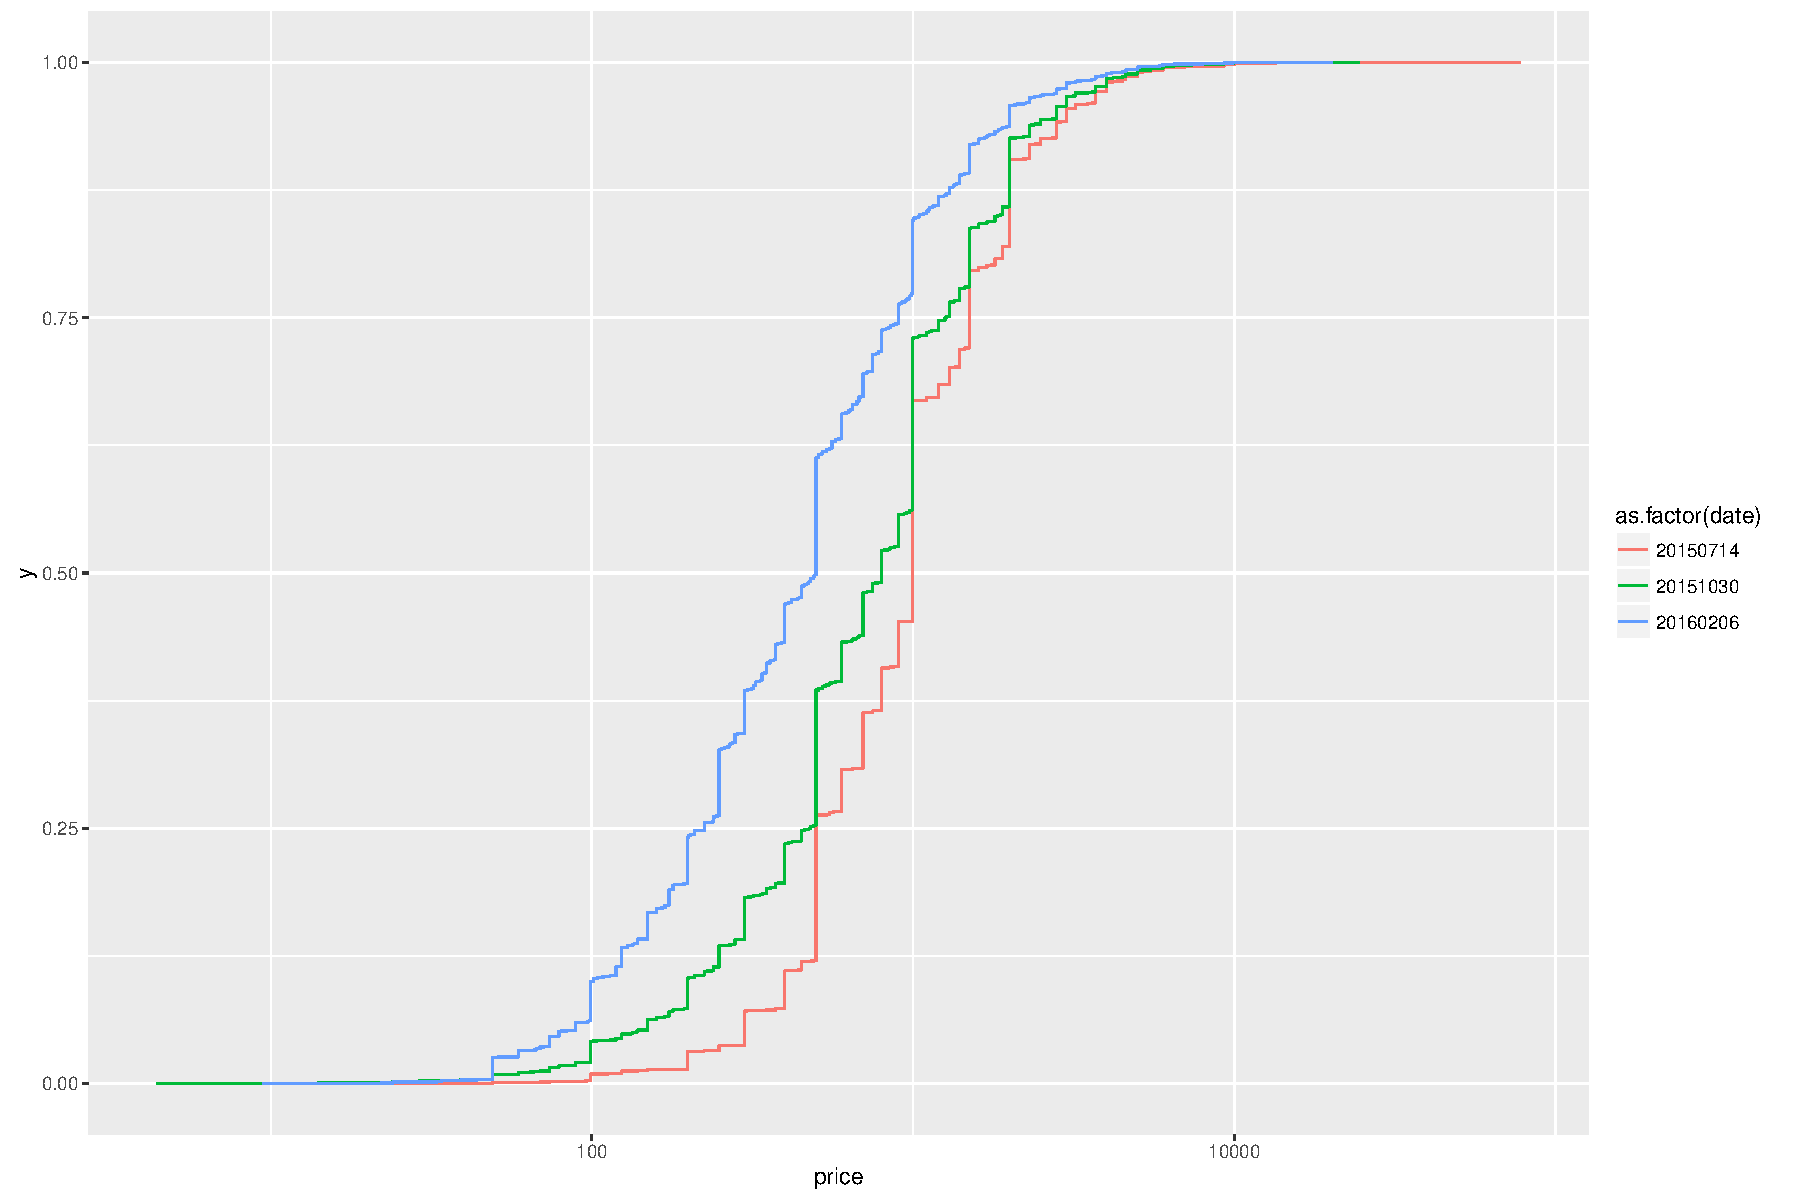
\includegraphics[width=1.0\columnwidth]{images/steam-prices.pdf}
%	\caption{CDF of games on the \steam platform at three distinct dates. The February data was collected in a sales period.}
%\label{fig:steam-prices}
%\end{figure}

This was combined with \acrshort{API}-data from the 3rd-party Web site SteamSpy\footnote{\url{https://steamspy.com}}. This site parses the portion of publicly visible \steam user profiles and from this estimates statistics on the size of the playerbase and the time each player spends with a title. Furthermore, the site provides a heuristic projection of the total number of owners of each listed title on \steam. Using this data also immediately makes evident a relationship between the price category of a game and the average time it's being played (cf. Fig.~\ref{fig:steam-cost-vs-playtime-violin}). Free (but especially free-to-play titles with monetization options other than an upfront payment) titles seem to occupy a special position as no prevalence for specific playtimes is visible. 

%\todo[inline]{Ist ``free'' auch in-app Purchase Zeug?}
%\todo[inline]{FM: This includes everything without any upfront costs: free, free-to-play with microtransactions, free to install but with subscriptions, ...}


\begin{figure}[!t]
	\centering
	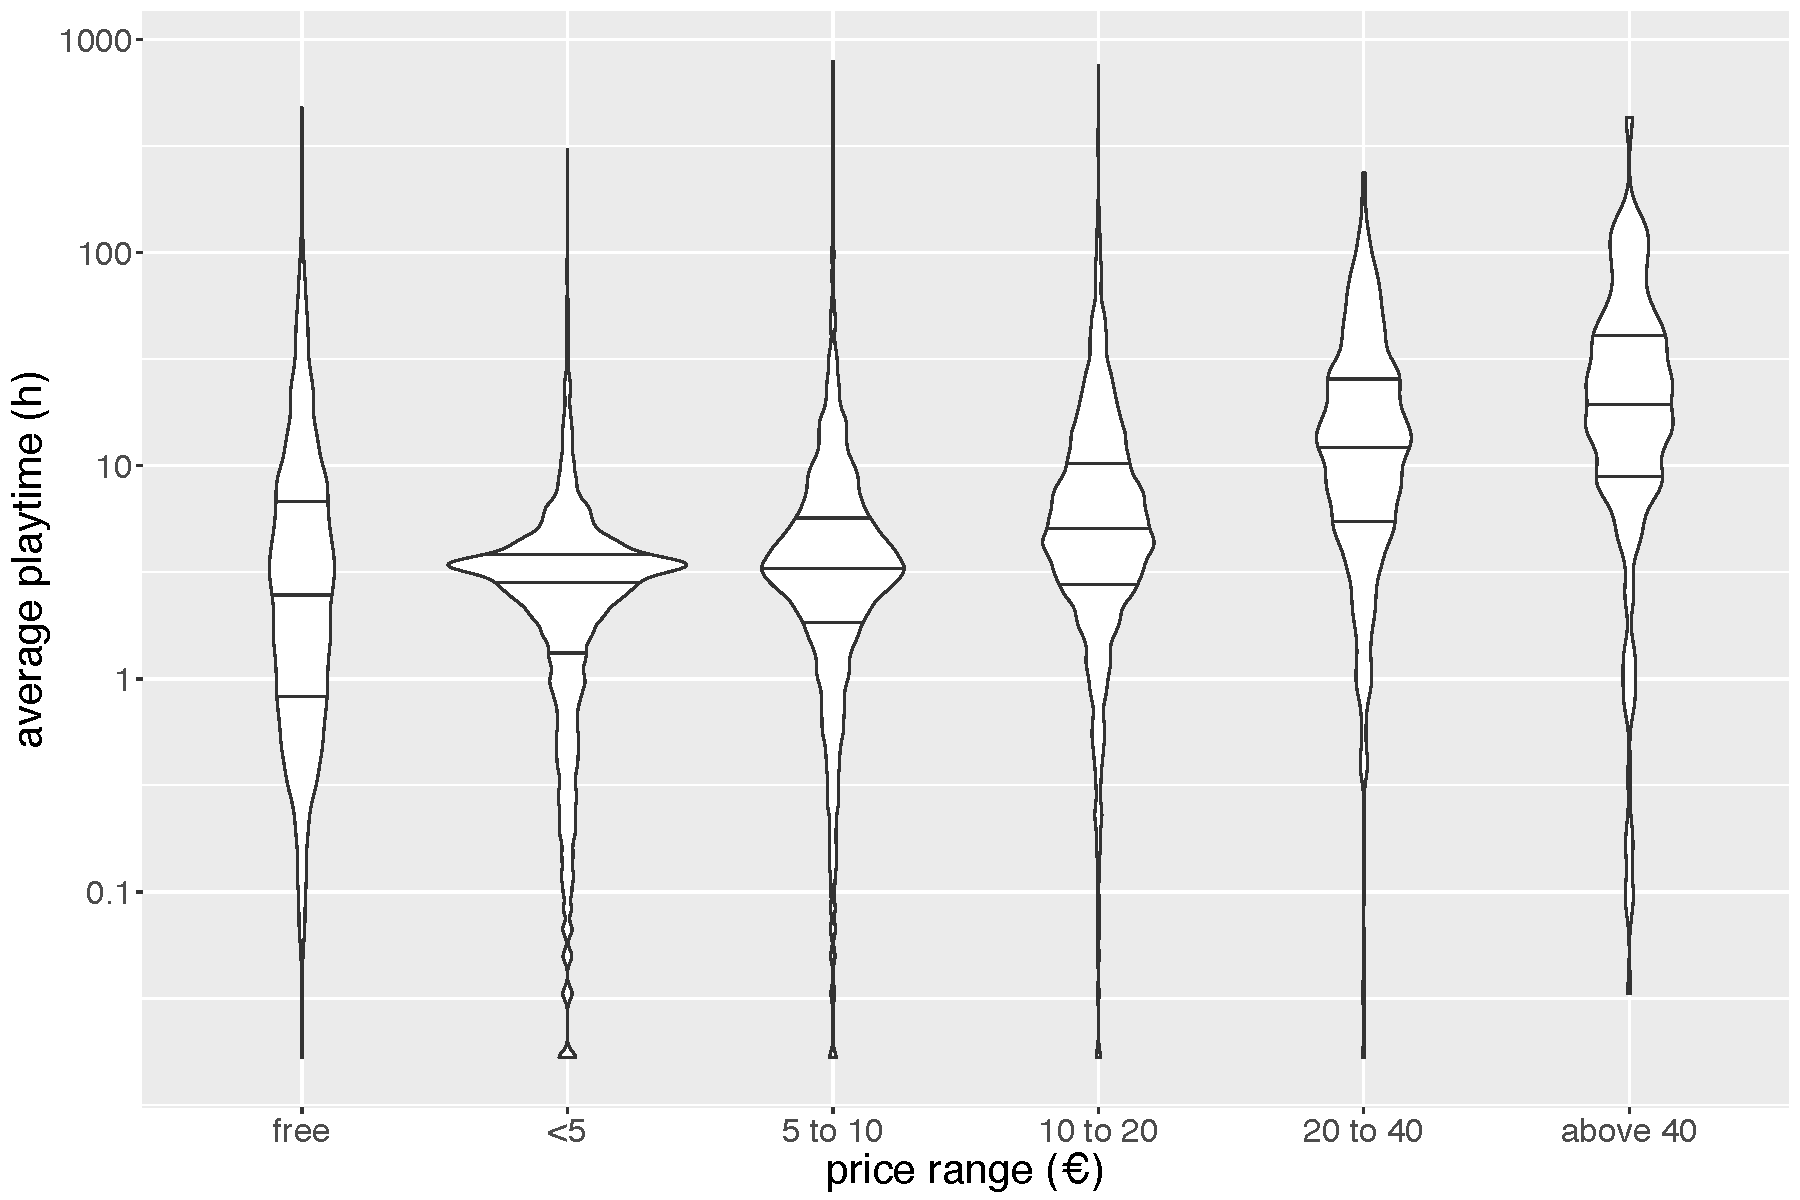
\includegraphics[width=1.0\columnwidth]{images/steam-cost-vs-playtime-non-sale.pdf}
	\caption{Violin plot of the average playtime of \steam games, broadly categorized by their prices. The number of games per bin are roughly $1$\si{\kilo}, $2$\si{\kilo}, $2$\si{\kilo}, $1$\si{\kilo}, $300$, and $90$.}
\label{fig:steam-cost-vs-playtime-violin}
\end{figure}



Due to the strong popularity of \steam in PC gaming (even physical retail copies often require using the service nowadays) this set also gives a good general overview of the dimensions of PC gaming in general.


%%%%%%%%%%%%
\subsubsection{Review Scores}


A final indirect measure of value and user satisfaction are review score as given by professional gaming media outlets. The largest dataset of such scores is available through Metacritic\footnote{\url{http://www.metacritic.com/}}, which is included in the present analysis\footnote{\url{https://github.com/mas-ude/metacritic_scraper}}.
\todo[inline]{We only use the script, right.. maybe add clarification in footnote? Does the set really cover ``all'' plattforms?}

This set covers all current and historic gaming platforms. The review scores are aggregated to average scores ranging between $0$ and $100$. Some internal weighing factors are applied that  signify the importance of some media outlets over others.

The exact release date of every title is also included, leading to another possible engagement metric: the game's age. Barring some highly favored classic titles, more recent games are usually much more popular than older ones.


% TODO: include or compare with data from opencritic.com as soon as their API is public/usable

% \begin{figure}[!t]
% 	\centering
% 	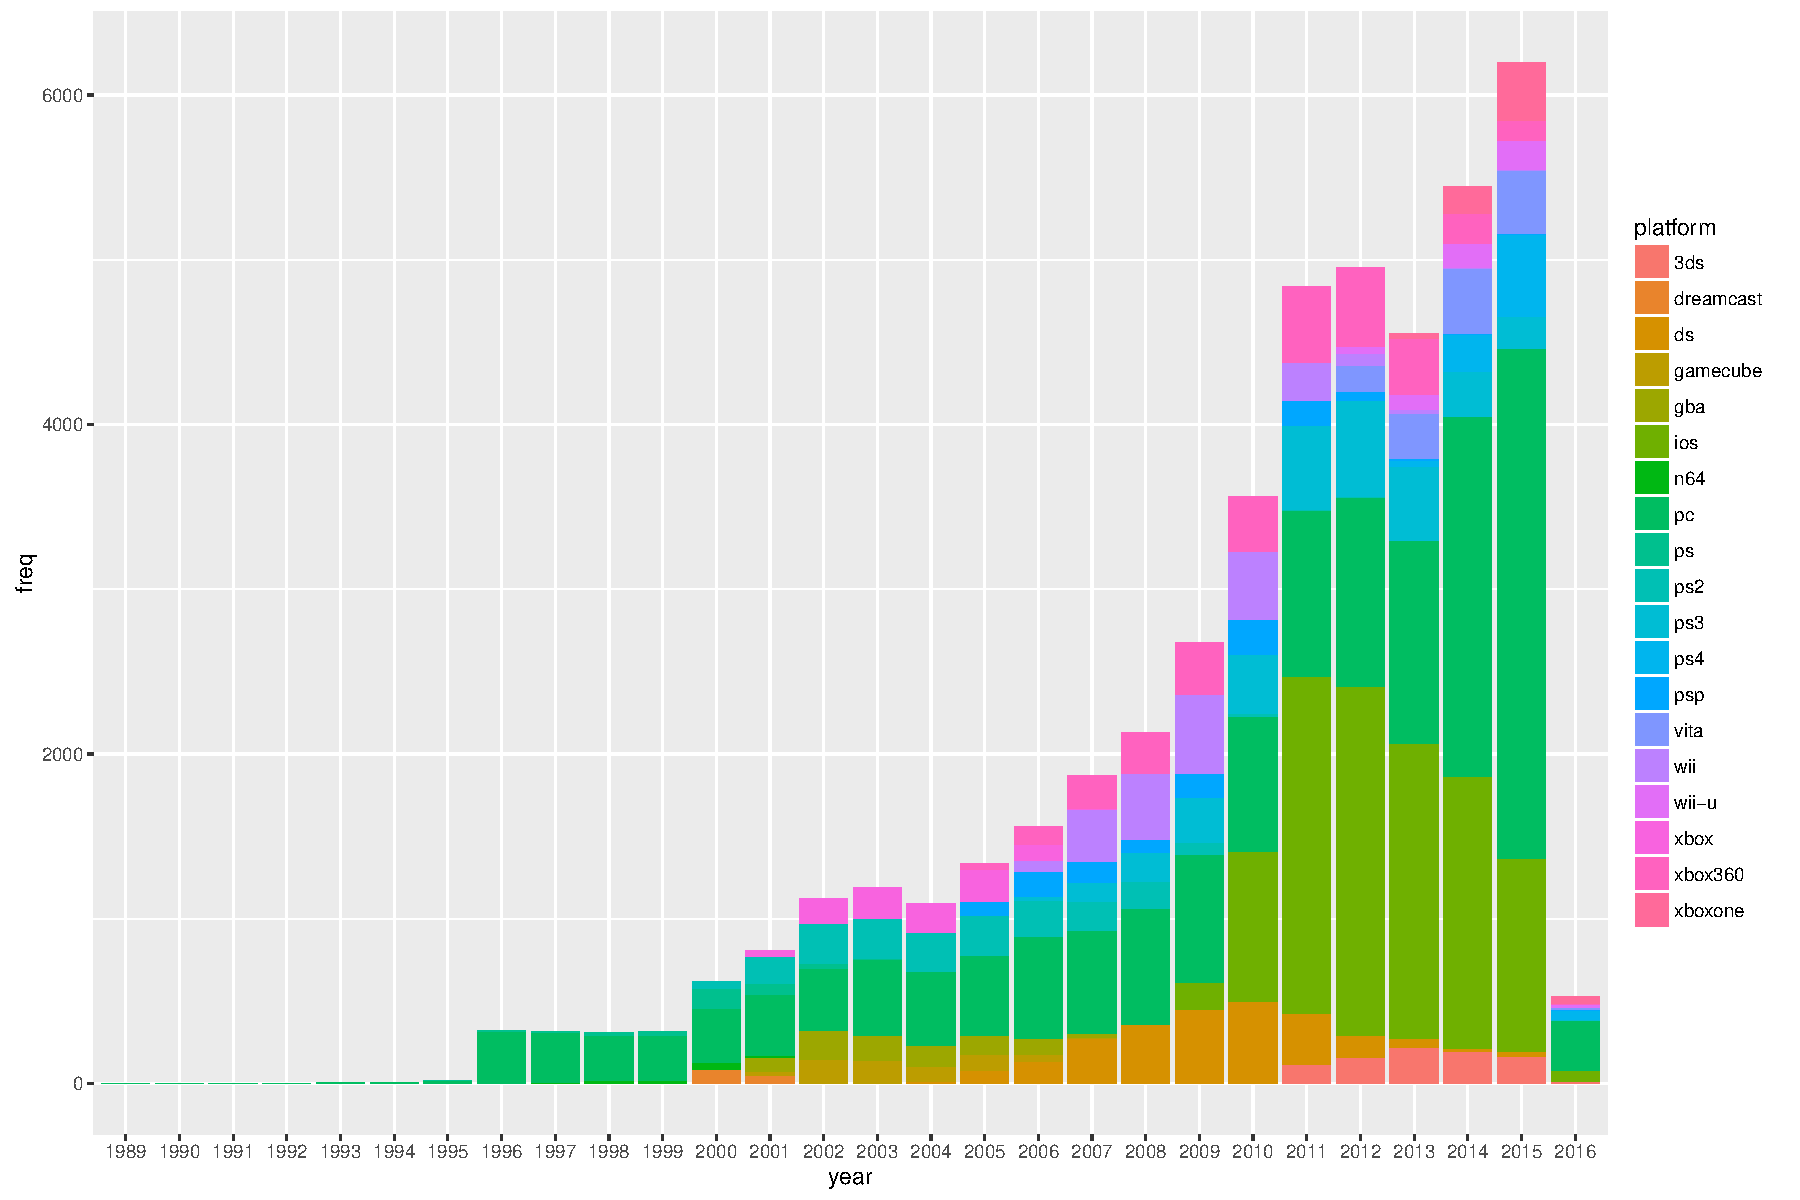
\includegraphics[width=1.0\columnwidth]{images/releases-per-year.pdf}
% 	\caption{Number of game releases per platform according to the Metacritic data.}
% \label{fig:releases-per-year}
% \end{figure}




